\documentclass[crop,tikz]{standalone}

\usepackage{makecell}

\definecolor{alizarin}{rgb}{0.82, 0.1, 0.26}
\definecolor{airforceblue}{rgb}{0.36, 0.54, 0.66}
\definecolor{apricot}{rgb}{0.98, 0.81, 0.69}
\definecolor{blush}{rgb}{0.87, 0.36, 0.51}
\definecolor{cadmiumgreen}{rgb}{0.0, 0.42, 0.24}
\definecolor{cambridgeblue}{rgb}{0.64, 0.76, 0.68}
\definecolor{celadon}{rgb}{0.67, 0.88, 0.69}
\definecolor{chestnut}{rgb}{0.8, 0.36, 0.36}
\definecolor{harvardcrimson}{rgb}{0.79, 0.0, 0.09}
\definecolor{darkseagreen}{rgb}{0.56, 0.74, 0.56}
\definecolor{aoenglish}{rgb}{0.0, 0.5, 0.0}
\definecolor{brightube}{rgb}{0.82, 0.62, 0.91}
\definecolor{amethyst}{rgb}{0.6, 0.4, 0.8}
\definecolor{asparagus}{rgb}{0.53, 0.66, 0.42}

\usetikzlibrary{positioning}
\usetikzlibrary{matrix}
\usetikzlibrary{fit}
\usetikzlibrary{calc,decorations.pathmorphing,patterns}
\usetikzlibrary{decorations.pathreplacing}


\newcommand{\vvector}[1]{\tikz{\draw[#1,step=1em,fill=#1!50] (0,0)  grid (1em,4em) rectangle (0, 0);}}
\newcommand{\hvector}[1]{\tikz{\draw[#1,step=1em,fill=#1!50] (0,0)  grid (4em,1em) rectangle (0, 0);}}
\newcommand{\vvectorSmall}[1]{\tikz{\draw[#1,step=.5em,fill=#1!50] (0,0)  grid (.5em,1.5em) rectangle (0, 0);}}

\newdimen\XCoord
\newdimen\YCoord
\newdimen\XXCoord
\newdimen\YYCoord

\newdimen\empty
\newdimen\fromX
\newdimen\fromY
\newdimen\toX
\newdimen\toY

\newcommand{\outgoing}[2]{
  \path (#1); \pgfgetlastxy{\XCoord}{\YCoord};
  \path (#2); \pgfgetlastxy{\XXCoord}{\YYCoord};
  \draw[->, line width=1pt] (\XCoord, \YCoord) -- (\XCoord, \YYCoord);
}%
\newcommand{\incoming}[2]{
  \path (#1); \pgfgetlastxy{\XCoord}{\YCoord};
  \path (#2); \pgfgetlastxy{\XXCoord}{\YYCoord};
  \draw[->, line width=1pt] (\XCoord, \YYCoord) -- (\XCoord, \YCoord);
}%
% horizontal arrow: (#1.x, #3.y) -- (#2.x, #3.y)
\newcommand{\horizontalArrow}[3]{
  \path (#1); \pgfgetlastxy{\fromX}{\empty};
  \path (#2); \pgfgetlastxy{\toX}{\empty};
  \path (#3); \pgfgetlastxy{\empty}{\fromY};
  \draw[->, line width=1pt] (\fromX, \fromY) -- (\toX, \fromY);
}%
% vertical braces: (#3.x, #1.y) -- (#3.x, #2.y)
\newcommand{\verticalBraces}[4]{
  \path (#1); \pgfgetlastxy{\empty}{\fromY};
  \path (#2); \pgfgetlastxy{\empty}{\toY};
  \path (#3); \pgfgetlastxy{\fromX}{\empty};
  % XXX the values for positionning the node for #4 have been choosen for the NMT example. must be checked
  \draw [decorate,decoration={brace,amplitude=3pt,raise=4pt},yshift=0pt] (\fromX, \fromY) -- (\fromX, \toY) node [midway, anchor=west, xshift=.2cm] {#4};
}%


\usepackage{tikz-dependency}
%\usepackage{verbatimbox}

\begin{document}

%\begin{myverbbox}{\amrText}

%\end{myverbbox}


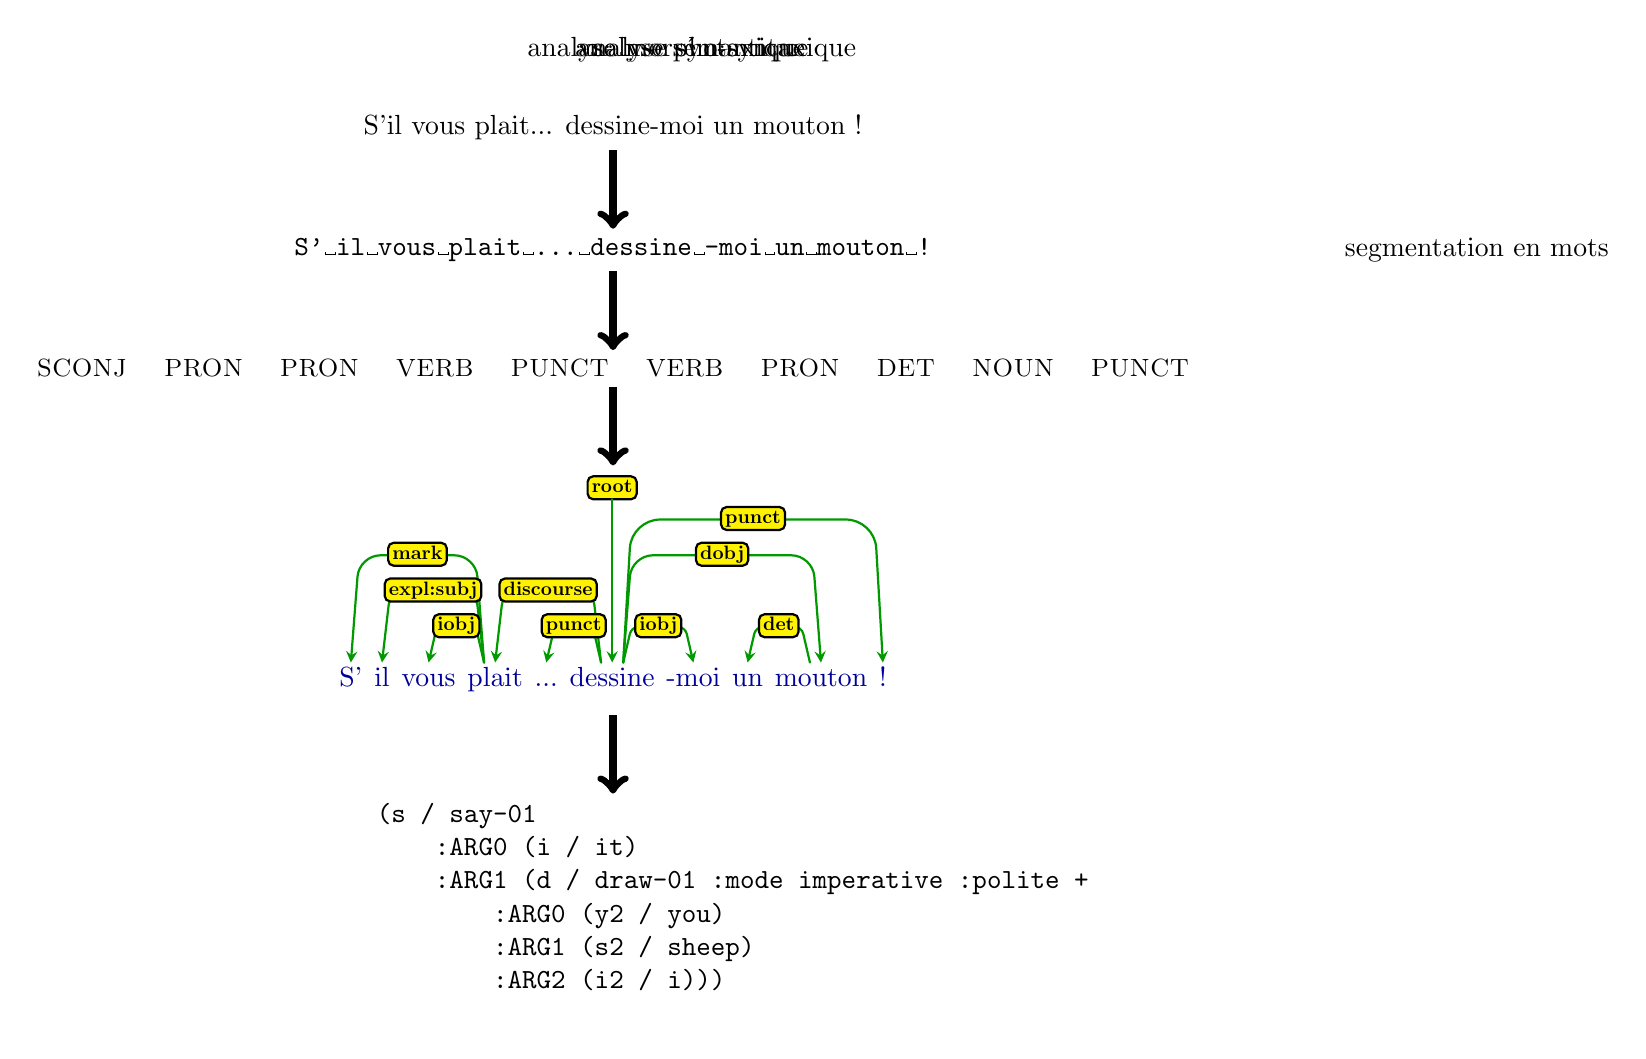
\begin{tikzpicture}

    \node (sentence) {S'il vous plait... dessine-moi un mouton !};

    \node (tokens) [below=of sentence] {\texttt{S'\textvisiblespace{}il\textvisiblespace{}vous\textvisiblespace{}plait\textvisiblespace{}...\textvisiblespace{}dessine\textvisiblespace{}-moi\textvisiblespace{}un\textvisiblespace{}mouton\textvisiblespace{}!}};

    \node (pos) [below=of tokens] {\small \textsc{SCONJ \quad PRON \quad PRON \quad VERB \quad PUNCT \quad VERB \quad PRON \quad DET \quad NOUN \quad PUNCT}};

    \node (parse) [below=of pos]{
        \begin{dependency}[theme=brazil]
            \begin{deptext}
                S' \& il \& vous \& plait \& ... \& dessine \& -moi \& un \& mouton \&! \\
            \end{deptext}
        
            \depedge{4}{1}{mark}
            \depedge{4}{2}{expl:subj}
            \depedge{4}{3}{iobj}
            \depedge{6}{4}{discourse}
            \depedge{6}{5}{punct}
            \depedge{6}{7}{iobj}
            \depedge{6}{9}{dobj}
            \depedge{6}{10}{punct}
            \depedge{9}{8}{det}
            \deproot[edge unit distance=4ex]{6}{root}
        \end{dependency}
    };

    \node (amr) [below=of parse] {
        \begin{minipage}{6cm}
            \begin{verbatim}
(s / say-01
    :ARG0 (i / it)
    :ARG1 (d / draw-01 :mode imperative :polite +
        :ARG0 (y2 / you)
        :ARG1 (s2 / sheep)
        :ARG2 (i2 / i)))
            \end{verbatim}
        \end{minipage}
    };

    \draw[line width=1mm, ->] (sentence) -- (tokens);
    \draw[line width=1mm, ->] (tokens) -- (pos);
    \draw[line width=1mm, ->] (pos) -- (parse);
    \draw[line width=1mm, ->] (parse) -- (amr);

    \node (label1) [right=5cm of tokens] {segmentation en mots};

    \GetXCoord{label1}{center}
    \GetYCoord{pos}{center}
    \node (label2) at (\myx,\myy) {analyse morpho-syntaxique};

    \GetXCoord{label1}{center}
    \GetYCoord{parse}{center}
    \node (label3) at (\myx,\myy) {analyse syntaxique};

    \GetXCoord{label1}{center}
    \GetYCoord{amr}{center}
    \node (label4) at (\myx,\myy) {analyse sémantique};

\end{tikzpicture}

\end{document}